% !TEX root = ../main.tex
% TODO: GENERAL CHECKUP NEEDED

\section{Nomad Kin}
\begin{linenumbers}
\DndDropCapLine{O}{utsiders, the lot of them. Dragged}
\textit{into our world by an unnatural pull, ever unable to find stable footing.
No matter how much they beg and cry, do not allow them into your home.
Touched by a strange flame, whose brightness attracts equally as strange beasts into your door, into your hearth.
Get rid of them before they share their misfortune with you.}

\hspace*{\fill} --- Abneh, renowned nimrod.

Brought into this world with the Schism, the nomad kin are a strange race from the outer lands.
Also known as umans, they have almost hairless bodies, and are similar in appearance to apes.

For an unknown reason, umans attract all kinds of predators from these lands.
Additionally, their blood has similar properties to the tall ones', and is used in many rituals.
Because of these reasons, umans are dispersed all around the world, and are nomadic in nature.

\subsection*{A Broad Spectrum}
Hunted by all kinds of kin and creatures, the nomad kin are forced to perpetually migrate and adapt to different environments, making them more physically diverse than the common kins.

There is no typical uman, with an individual standing from 1.5 meters to a little over 1.8 meters tall, and weighing from 60 to 125 kgs.
Acclimating to even the most extreme environments, a uman's skin shades to any color from the darkest brown to the lightest hues.
They also grow long hair in their scalps and faces, sporting a great variety of colors and thickness.
Nomads reach adulthood at around 14, and rarely live a single century.

Umans are a gendered kin, and usually have one child at a time.
Families consist of a father, a mother, and their kid or children, but it is not uncommon for other members of the nomadic groups to care for parentless children.

\subsection*{Accursed Coldblood}
Known as coldblood due to its cerulean tint, Umans' blood has special properties, and is very useful for spellcasters.
It retains a sort of energy, and can be used as a source of spells.
Umans know this, and regularly prepare blood vials for trade and to strengthen troupes' wizards.

Umans pay dearly for this special blood, as it acts as a beacon for the predators from the outer lands, the coldblood beasts.
These creatures hunt umans, and many of the kin are banned from villages for safety concerns.

Spellcasters seek coldblood, and many try to attain it by any means available.
Naturally, the murder of umans for their blood is illegal in most nations, but some carry the custom on nevertheless.
The nimrods are a cult that specializes in gathering coldblood via any means available, and are commonly contracted by wizards and warlocks to attain the product.

\subsection*{Adaptable and Durable}
Hunted by both beast and kin, umans have trouble trusting others and don't normally settle in communities of other kins.
They live in troupes exclusive to their kin, where usually all members have some familiar relationship.
Troupes travel together and care for each other, assigning specific roles to each member based on their skills.

Far from vulnerable, most troupes are fierce and resilient, hardened by centuries of being preyed upon.
Groups keep track of how they are treated by different cities and towns, and only do commerce where they are accepted.

While uncommon, some uman communities have managed to settle in one place.
These communities keep their locations secret, communicating it only to other umans via traveller's cant, a set of writings and symbols they brought from the outer lands.

\subsection*{Life in Escapade}
For a uman, a life of adventure is not a romantic desire but rather a fact of mundane life.
Used to the hardships of survival, a uman is especially capable of fending off threats and surpassing hardships.

It is very common to see lone uman adventurers, either as exiles or in a quest for their troupe.
Whatever the motive, they naturally excel at voyages, and are a great fit on any adventuring party.

\subsection*{Uman Names}
Umans most commonly wear names from other cultures.
Even in the outer lands, umans were known to have a great variety of names depending on each specific culture.
Those who desire to conserve their roots choose old names from their history and legends to give their children.

\paragraph{Common Names}
(Male) Anton, Aseir, Diero, Dorn, Evendur, Grim, Haseid, Ivor, Khemed, Kosef, Marcon, Morn, Pavel, Pieron, Rimardo, Romero, Salazar, Sergor, Umbero, Zasheir;
(female) Atala, Arveene, Balama, Ceidil, Chessail, Dona, Faila, Jasmal, Luisa, Lureene, Marta, Quara, Rowan, Seipora, Selise, Shandri, Vonda;
(surnames) Agosto, Amblecrown, Astorio, Basha, Buckman, Calabra, Domine, Evenwood, Falone, Greycastle, Khalid, Kulenov, Marivaldi, Marsk, Nemetsk, Pashar, Pisacar, Ramondo, Rein, Starag.

\paragraph{Frostburn Names}
(Male) Ander, Blath, Bran, Frath, Geth, Lander, Luth, Malcer, Stor, Taman, Urth;
(female) Amafrey, Betha, Cefrey, Kethra, Mara, Olga, Silifrey, Westra;
(surnames) Brightwood, Helder, Hornraven, Lackman, Stormwind, Windrivver.

\paragraph{Boggart Names}
(Male) Aoth, Bareris, Ehput-Ki, Kethoth, Mumed, Ramas, So-Kehur, Thazar-De, Urhur;
(female) Arizima, Chathi, Nephis, Nulara, Murithi, Sefris, Thola, Umara, Zolis;
(surnames) Ankhalab, Anskuld, Fezim, Hahpet, Nathandem, Sepret, Uuthrakt.

\begin{figure}[!b]
    \centering
    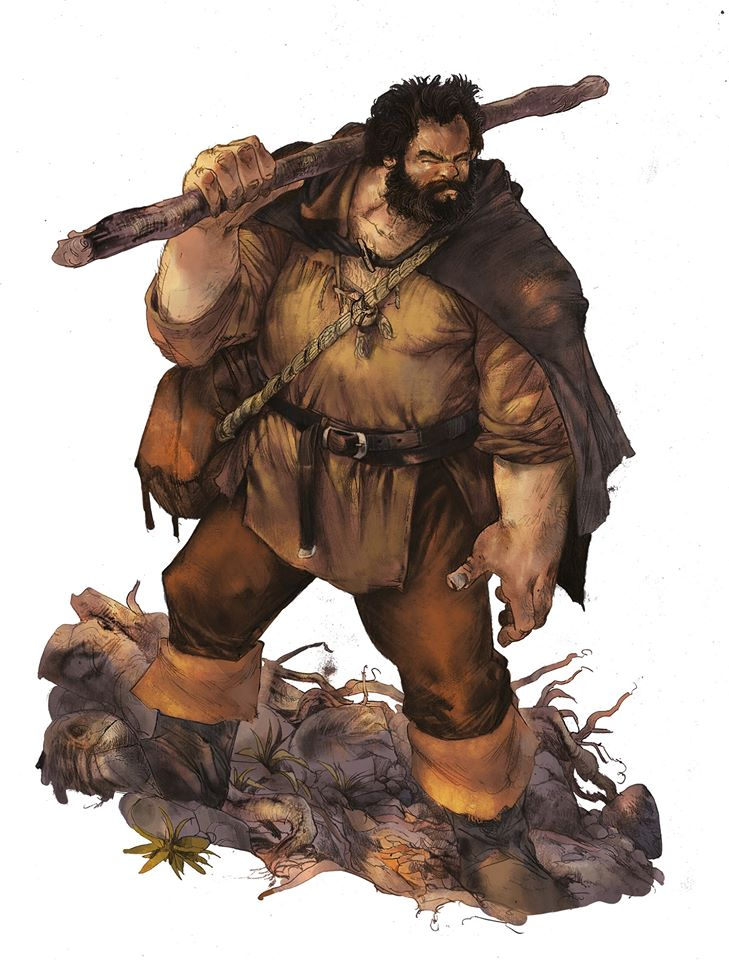
\includegraphics[width=0.48\textwidth]{02kins/img/19uman_monk.jpg}
\end{figure}

\subsection*{Traits}
The nomad kin is known for their survival and adaptability, and your uman character receives the following traits:
\subparagraph{Ability Score Increase} Two different ability scores of your choice are increased by 1.
\subparagraph{Age} Umans reach adulthood in their late teens and live less than a century, if they manage to survive that long.
\subparagraph{Alignment} Umans tend to no particular alignment, but they do have a penchant for community and justice, and tend to the indigo tide.
\subparagraph{Size} Umans vary widely in height and build, from barely 1.5 meters to well over 1.8 meters tall.
Regardless of your position in that range, your size is Medium.
\subparagraph{Speed} Your base walking speed is 9 meters.
\subparagraph{Languages} You can speak, read, and write the nomad tongue, and an additional language of your choice.
You can also read and write the traveller's cant, a set of writings and symbols created by your kin to help and communicate with each other.
\subparagraph{Learned Durability} You gain proficiency in the Survival skill.
\subparagraph{Relentless Endurance} When you are reduced to 0 hit points but not killed outright, you can drop to 1 hit points instead.
You can't use this feature again until you finish a long rest.

\begin{figure}[!t]
    \centering
    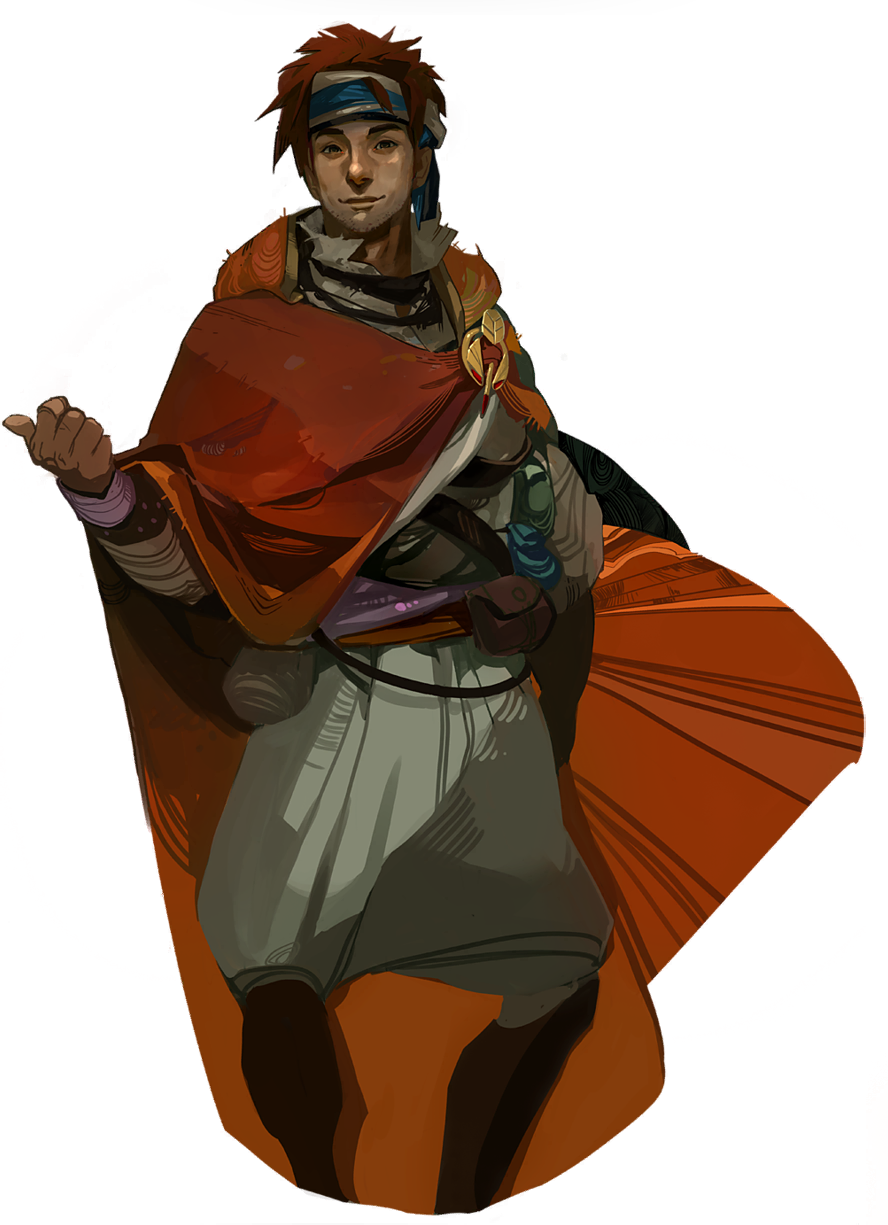
\includegraphics[width=0.48\textwidth]{02kins/img/19uman_nomad.png}
\end{figure}

\subsubsection{Common Nomad}
While umans are known to be extremely adaptable to extreme habitats, most don't stay at one place for enough time to acquire this specialty and remain, for lack of a better word, common.
In stark contrast with their name, each of these umans is unique and as such your features are specially dynamic.
\subparagraph{Languages} You can read, write and speak one additional language of your choice.
\subparagraph{Skills} You gain proficiency in one skill of your choice.
\subparagraph{Trained} You gain proficiency with one simple or martial weapon of your choice.
\subparagraph{Handy} You are proficient with a set of artisan's tools of your choice.
\subparagraph{Feat} You gain one feat of your choice.

\subsubsection{Frostburn Nomad}
With skins ranging from pale blue to light purple, and hair shades from the lightest of white to deep brown colors, the Frostburn are a kin that comes from a troupe of umans that managed to survive in the lands beyond the wall of ice and stone, and beyond the reach of most coldblood beasts and nimrods.
%These umans tend to dress with the bones and furs of the creatures they hunt, using their inventiveness to craft clothing to intimidate and scare rather than protect against cold, since their thick skins already manage this task effortlessly.
\subparagraph{Ability Score Increase} Your Constitution score is increased by 1.
\subparagraph{Menacing} You are naturally proficient in the intimidation skill.
\subparagraph{Born Hunter} You are proficient with clubs, daggers, spears, and barbed spears.
\subparagraph{Thick Skin} %You are naturally acclimated to cold environments and don't need sources of heat to survive in all but the most extreme cold.
You are resistant to cold damage.%, and remain unaffected by cold environments.
\subparagraph{Ice Shell} Once per short rest, you can grow a thick layer of ice around your body to protect you.
You gain resistance to piercing and slashing damage, and vulnerability to bludgeoning damage for a number of turns equal to your Constitution modifier (Minimum of 1).
Additionally, any creature that attacks you with a melee attack during this time suffers 1d4 piercing damage.

\subsubsection{Boggart}
Boggarts are umans that live in the swamps and marshes of Yuadrem.
Boggarts are generally tall, slim, and amber-skinned, with eyes of hazel or brown.
Their hair ranges from black to dark brown, but most shave off all their hair.
These umans are craftier than the average, and are known to prepare complex traps and mechanisms to protect their communities or alert them of imminent danger.
\subparagraph{Ability Score Increase} Your Wisdom score is increased by 1.
\subparagraph{Bog Swimmer} Boggart tactics usually include a good dose of swimming through less than cooperative waters.
You have a swimming speed of 7.5 meters.
\subparagraph{Swamp Life} You have advantage on saving throws against poison and diseases, and you have resistance against poison damage.
\subparagraph{Stealthy Hunter} You have proficiency with blowguns, nets, and bolas.
You also are proficient with a Poisoner's kit.

\subsubsection{Cursed Kin}
It is said that the umans who remain in the place of their arrival start showing their true form.
While the accuracy of this statement remains untested, it is true that those who stay in the forbidden lands do show strange changes to their appearance.
Large, black horns grow on their heads, their skin and eyes turn into a very pale shade, and their bodies grow.
While most cursed kin do act more menacing and violent than the average uman, it is likely that this is a side effect of their harsh homeland more than a natural development in their minds.
\subparagraph{Size} Unlike most nomad kin, you stand between 2.1 and 2.4 meters tall and weight between 140 and 170 kg.
Your size is medium.
\subparagraph{Ability Score Increase} Your Strength score is increased by 1.
\subparagraph{Natural Athlete} You have proficiency in the Athletics skill.
% \subparagraph{Abyssal Resistance} You have resistance to fire damage.
\subparagraph{Unholy Fortitude} Your hit point maximum increases by an amount equal to your level (minimum 1).
\subparagraph{Ram} Your horns are a natural weapon, which you may use use to make unarmed strikes.
If you hit with them, you deal bludgeoning damage equal to 1d4 + your Strength modifier, instead of the damage normal for an unarmed strike.
\subparagraph{Powerful Build} You count as one size larger when determining your carrying capacity and the weight you can push, drag or lift.

\begin{figure}[!b]
    \centering
    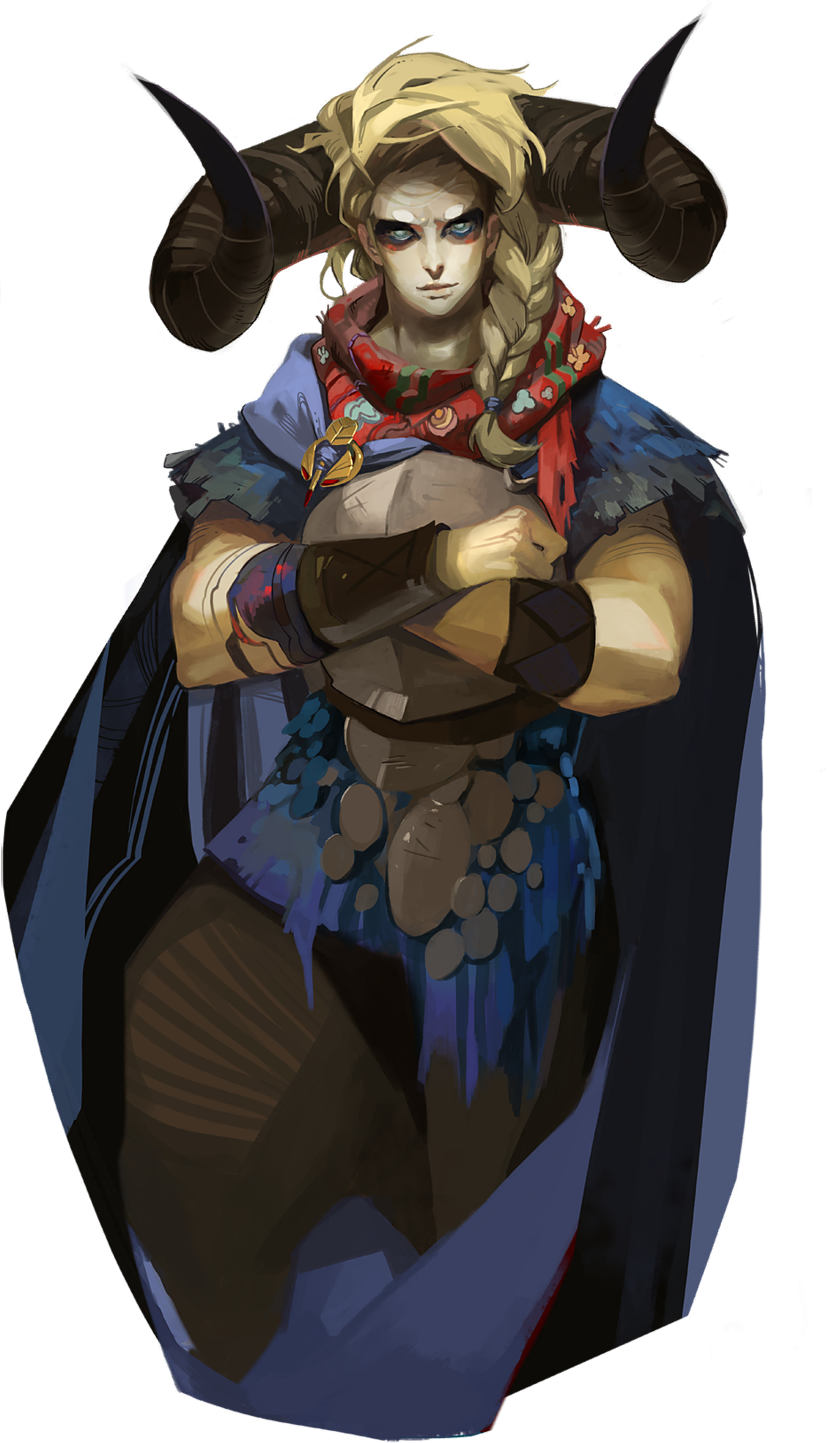
\includegraphics[width=0.48\textwidth]{02kins/img/19uman_cursed.png}
\end{figure}
\end{linenumbers}
